\section{ThingSat}
\label{sec:case-study}

\subsection{Overview}
% \paragraph*{Mission Goal:} in-orbit observation of glaciers in Europe and in Polynesia.
% \paragraph*{Approach}: rent "rack" space as payload on a CubeSat (SatRevolution).

%----important
% citation --> Antenna : technical report
%----secondary
% Stork mission (404) : https://web.archive.org/web/20210420173051/https://satrevolution.com/products/stork-mission/
%in comparison to other project a GW in the sky not just a ping
% Sat-IoT

% Most of the earth’s surface lack of terrestrial networks. These zones include
% populated areas that necessitate technologies to permit communication with more
% connected areas, enable scientists to have networks in wild areas (e.g. Polar
% zones and oceans) to support their research, monitor isolated beacons and
% prevent of risks. Solutions have been developed in the last decades, notably the
% LoRa technology, that facilitate a long range communication with a low power
% consumption for IoT (Internet of things). 

The goal of the ThingSat project is to benchmark direct LoRa communications
between a LEO (Low Earth Orbit) cubesat and nodes on the ground (end-devices
(ED) or ground stations (GS)). We designed an electronical board with its
antenna that is the guest payload of a shared 3U CubeSat -
\href{https://space.skyrocket.de/doc_sdat/stork-1.htm}{STORK-1} from the polish
start-up \href{https://www.satrevolution.com/}{SatRevolution}. The cubesat was
launched on a near-polar orbit at an altitude of 520 km on January 13th, 2022. 

\begin{figure}[ht]
    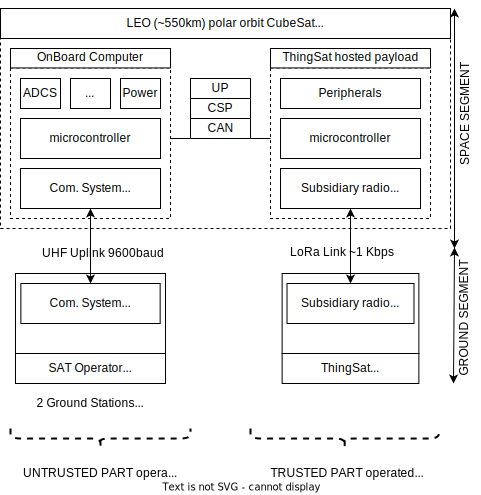
\includegraphics[width=0.5\textwidth]{Figures/globecom-thingsat.jpg}
    \caption{The cubesat ecosystem}
    \label{fig:archi}
\end{figure}

% \paragraph*{High-level overview of Segments}

The figure \ref{fig:archi} generalizes the Thingsat context by giving an
overview of a cubesat ecosystem where the interaction with a hosted payload go
through an unstrusted part.

\subsection{Distributed System Architecture}

\paragraph*{Space Segment Description}

The OnBoard Computer consists of a microcontroller with all its subsystems to
operate the cubesat : the Attitude Determination and Control System, the
communication subsystems (UHF/VHF/S-band for uplink/downlink + antennas),
the power subsystem (Battery Management, Energy Harvesting with Solar Panels,
Auxiliary Power Supply). 

The payload designed for the Thingsat project embeds one
\href{https://www.semtech.com/products/wireless-rf/lora-gateways/sx1302}{Semtech
SX1302 concentrator} for communications on the 863-870 MHz band and one
\href{https://www.semtech.com/products/wireless-rf/24-ghz-transceivers/sx1280}{Semtech
SX1280 transceiver} for communications on the 2400-2500 MHz band. Each
transceiver is controlled by its own STM32 microcontroller. The firmware of both
microcontrollers is developed with \href{https://github.com/RIOT-OS/RIOT}{RIOT
OS}. Furthermore a dual-band patch antenna (868MHz, 2.4GHz) was designed.

\paragraph*{Ground Segment Description}
% \paragraph*{Control Segment} % Francisco: not sure if its the right name

For the ground segment, the cubesat operator relies on i) ground
stations\footnote{not necessarily owned by the cubesat operator} to communicate
with the OBC and ii) a Command \& Control Center to operate the cubesat
(telecommand/telemetry) and to provide a means for payload maintainers to
interact with the hosted payload.

\paragraph*{OBC \& Payload Communication Bus}

\paragraph*{Payload Description}: tenant status, energy budget, on time etc.
% - OBC -> SatRev controlled
% - Payload -> Full Control

\subsection{Communication Characteristics Overview}
\paragraph*{link-budget Mission Control}: delivering and communicating mission
files, delivering software updates, latency, etc.

Typical polar LEO satellites carry out an average of 2-4 passes over one ground
station. The duration of the communication window is approximately of 5 to 10
minutes. Communication with cubesats are generally done on amateur frequency
bands (UHF/VHF) with very average low data rates ranging from 9.6kbps to
100kbps. With only 2 ground stations to interact with the cubesat and a 10-kbps
link, the data that can be exchanged during a day is roughly 1500KB (= 2 GS x 2
passes/day x 5-min pass x 10kbps). This amount should be divided among OBC
(telecommand/telemetry/update) and hosted payload communications. To give an
order of idea, the Thingsat payload benefits from 300KB per day. 

The data exchanged by the Payload Maintainer with the Thingsat payload comprises 
\begin{itemize}
    \item the delivery of mission files runnng above the same firmware and the
    recovery of experiment results
    \item firmware updates
    \item diagnostic files to help the debug of failed missions/updates
\end{itemize} 

\paragraph*{link-budget Mission}: communication between OBC and Payload, payload
active time for communication with ground segments.

Regarding the communication with the OBC, an API is provided to the hosted
payload to read/write data with the data handling module of the cubesat as well
as interacting with its subsystems. To carry out a provisioned mission, the
payload needs information from the OBC : awaiting files, GPS,
time, ADCS, time before shutdown, ...

Furthermore the Thingsat payload is not active all the time as the power is only
enough for one payload at the same time. The mission of the STORK constellation
is earth observation. So each STORK cubesat is equipped with an
imager~\cite{wiki:SatRevolution} which has its own missions. Therefore the OBC
is in charge of turning on the relevant payload according to the schedule
uploaded from the ground. 

\subsection{Software Updates Requirements}
\paragraph*{What needs updates}: Missions ? 
\paragraph*{Why?}: timeline for deployment, CoVID context, etc. making it impossible
to deliver a fully functional device in time. Need to update the firmware remotely
and in orbit.
\paragraph*{Communication Chain}: how are new firmware, payloads delivered,
who has access, etc..
Regarding in-orbit software updates, the figure \ref{fig:archi} generalizes the
specific Thingsat context where hosted payload updates go through an unstrusted
part. Thus, a firmware (FW) update occurs as follows : i) the FW is uploaded to
the cubesat by the payload owner (PO) through one of the cubesat operator (CO)
ground stations (GS), ii) once the payload is turned on and reset, it asks
the OBC for any waiting file to execute, iii) the OBC uploads the FW chunk by
chunk to the payload and iv) the FW update process is triggered. 
